%% Copyright 2019 Bernd Haberstumpf
%% License: CC BY-NC
% !TeX spellcheck = de_DE
\newsection{Regelsystem}

Die Rollenspielregeln sind auf den narrativen Charakter des Plots ausgelegt. Es handelt sich um ein W6 W"urfelsystem bei dem vier W"urfel pro Spieler bzw.~den Spielleiter ausreichen. W"urfel legen dabei nicht die Eigenschaften einen Charakter im Detail fest oder beschreiben das Ergebnis einer Aktion, sondern spei\3en lediglich einen Zufallsfaktor in das Ergebnis ein. Das Ergebnis einer Aktion oder auch eines Ereignisses legt der Spielleiter unter Ber"ucksichtigung der Handlungen und des W"urfelergebnisses selbst fest. Das Regelsystem ist angelehnt an den Konzepten des Rollenspiels "`Blades in the Dark"'.


\newsection{W"urfelw"urfe}

Der Erfolg von Aktionen wird wie Beschrieben durch W"urfel beeinflusst werden. Das W"urfelergebins beschreibt wie erfolgreich eine Aktion gewesen ist. W"urfelw"urfe werden mit einem bis drei W6 W"urfeln ausgetragen. Das h"ochste W"urfelergebnis z"ahlt.

Es wird unterschieden zwischen \emph{Alltagswurf}, \emph{Einfacher Wurf}, \emph{Risikowurf} und \emph{Vergleichender Wurf}.

\newsubsection{Alltagswurf}
Ein Alltagswurf kann bei einer allt"aglichen Situation zum Einsatz kommen wie z.B. im ComNetz suchen. Bei einem Alltagswurf werden drei W"urfelerebnisse unterschieden:

\begin{diceroles}
    \sdice{1} & Die Aktion ist fehlgeschlagen und hat negative Auswirkungen auf den Ausf"uhrenden. \\
    \rdice{2}{5} & Die Aktion hatte Erfolg. \\
    \sdice{6} & Die Aktion hat einen herausragendes Erfolg. \\
\end{diceroles}

\begin{ruleexample}
    Rondra ist auf der Suche nach Informationen in einer einschl"agigen Disko. Sie begiebt sich auf die Tanzfl"ache. Der Spielleiter entscheidet sich f"ur einen W"urfelwurf. Rondra w"urfelt:

    \begin{diceroles}
        \sdice{1} & Rondra rempelt mehrere Discobesucher an und ger"at damit ins Visier der Security. \\
        \rdice{2}{5} & Rondra tanzt ungezwungen und kann dabei andere Discobesucher ansprechen. \\
        \sdice{6} & Rondra legt eine beeindruckende Performance aufs Parkett und erregt das Interesse des Barmanns Bruno 
            der ihr nur allzu gerne Antworten auf ihre Fragen gibt. \\
    \end{diceroles}
\end{ruleexample}

\newsubsection{Einfacher Wurf}
Ein einfacher Wurf beeinflusst das Ergebnis einer nicht allt"aglichen Herausforderung. Folgende W"urfelergebnisse werden unterschieden:

\begin{diceroles}
    \sdice{1} &  Die Aktion ist schwerwiegend fehlgeschlagen und hat negative Auswirkungen auf den der die Aktion ausf"uhren wollte.\\
    \rdice{2}{3} & Die Aktion hatte keinen Erfolg. \\
    \rdice{4}{5} & Die Aktion hatte einen Teilerfolg. \\
    \sdice{6} & Die Aktion hatte vollen Erfolg.\\
\end{diceroles}

\begin{ruleexample}
    Hektor ist auf der Suche nach Informationen im Raumhafen von Valhalla. Er wird von dem Agenten Johnson beschattet. Der Spielleiter l"asst den Spieler w"urfeln. Wird er den Agenten als solchen erkennen?

    \begin{diceroles}
        \sdice{1} & Der Agent rempelt Hektor unerkannt an und heftet ihm eine Nanowanze an den Overall.\\
        \rdice{2}{3} & Hektor bemerkt nichts.\\
        \rdice{5}{6} & Hektor bemerkt, dass er verfolgt wird verliert den Agenten zun"achst wieder aus den Augen.\\
        \sdice{6} & Hektor hat den Agenten entdeckt ohne das dieser seine Entdeckung bemerkt hat.\\
    \end{diceroles}
\end{ruleexample}

\newsubsection{Risikowurf}
Ein Risikowurf ist ein W"urfelwurf bei dem der W"urfelnde geringen Chancen auf Erfolg hat. Folgende W"urfelergebnisse kommen in Betracht:

\begin{diceroles}
    \sdice{1} & Die Aktion ist schwerwiegend fehlgeschlagen und hat negative Auswirkungen auf den der die Aktion ausf"uhren wollte.\\
    \rdice{2}{5} & Die Aktion hatte keinen Erfolg.\\
    \sdice{6} & Die Aktion hat einen Teilerfolg erzielt.\\
    \tdice{6}{6} & Die Aktion hat einen vollen Erfolg.\\
\end{diceroles}

\begin{ruleexample}
    In einem Raumgefecht erleidet Hektors Shuttle einen Schaden an der Man"ovriereinheit und taumelt durchs All. Haktor beschie\3t den Schaden an der Bordwand zu reparieren und verl"asst im Raumanzug das innere des Schiffs. Der Spielleiter l"asst w"urfeln:
    
    \begin{diceroles}
        \sdice{1} & Hektors Magnetstiefel verlieren die Haftung auf der Bordwand und Hektor schl"agt mit dem Kopf auf. Nun h"angt er  
            bewusstlos am Rettungsseil. Hoffentlich ist noch eine zweite Person an Bord, die ihn retten kann. \\
        \rdice{2}{5} & Hektor kann den Schaden nicht beheben.\\
        \sdice{6} & Hektor schafft es einen Teil der Steuereinheit notd"urftig zu reparieren. Hoffentlich reicht es das Schiff aus 
            der Schu\3linie zu bringen.\\
        \tdice{6}{6} & Hektor kann die Steuereinheit wieder vollst"andig in Betrieb nehmen.\\
    \end{diceroles}
\end{ruleexample}

\newsubsection{Vergleichender Wurf}
Bei einem vergleichenden Wurf kann das Ergebnis des ersten Wurfs durch einen Gegenwurf negativ beeinflusst werden. Ein vergleichender Wurf ist z.B. ein Angriff und eine Verteidigung. Der Angriffserfolg kann durch den verteidigenden Wurf abgeschw"acht werden. Erfolge eines verteidigenden Wurfs haben folgenden Einflu\3:

\begin{center}\begin{tabular}{m{1.2cm} m{1.2cm} m{11cm}}
    \textbf{Anriff} & \textbf{Vert.} & \textbf{Auswirkung} \\\hline
    Voll & Voll & Teilerfolg \\
    Voll & Teil & Minderung schwerer Folgen \\
    Teil & Voll & kein Erfolg \\
    Teil & Teil & Minderung Teilerfolg \\
\end{tabular}\end{center}

\begin{ruleexample}
    Hektor hat den Agenten Johnson potentiell im Raumhafen entdeckt. Johnson ist sich der Gefahr bewusst und will sich der Entdeckung entziehen. Der Spielleiter entscheidet sich f"ur einen vergleichenden Wurf.

    \begin{center}\begin{tabular}{m{1.2cm} m{1.2cm} m{11cm}}
        \textbf{Anriff} & \textbf{Vert.} & \textbf{Auswirkung} \\\hline
        Voll & Voll & Hektor bemerkt, dass er verfolgt verliert den Agenten aber wieder unerkannt aus den Augen.  \\
        Voll & Teil & Hektor hat den Agenten entdeckt, der Agent bemerkt, dass er aufgeflogen ist.\\
        Teil & Voll & Hektor bemerkt nichts. \\
        Teil & Teil & Hektor hat das Gef"uhl das er verfolgt wird. \\
    \end{tabular}\end{center}
\end{ruleexample}

\newsection{Der Charakter}\anchor{sec:character}

Die F"ahigkeiten und Eigenschaften eines Charakters sind neben den menschlichen Grundf"ahigkeiten durch seinen Hintergrund und spezielle St"arken und Schw"achen bestimmt. 

\begin{description}
    \item[Grundf"ahigkeiten] sind F"ahigkeiten die jeder Humanoiden mehr oder weniger beherrscht. Alles wof"ur keine spezielle Ausbildung,  
        kein spezielles ethnischer oder kulturelles Hintergrundwissen und keine speziellen K"orpereigenschaften ben"otigt werden f"allt in diese Kategorie. Jeder der es bis ins All geschafft hat kann Lesen schreiben und rechnen. Auch kann jeder eine entsicherte Feuerwaffen abfeuern. Auch k"onnen sich alle Bewohner der au\3erterrestrischen Kolonien miteinander irgendwie unterhalten. Gesprochen wird ein Kauderwelsch aus Englisch mit starken Einfl"ussen von Russisch, Chinesisch und Spanisch. Ausfl"uge mit einem Raumanzug ins All sind hingegen nicht selbstverst"andlich.  Aktionen in einer Grundf"ahigkeit werden mit \textbf{1W6} gew"urfelt. 
    \item[Hintergr"unde] beginnen mit einer Kulturkreis entsprechender Muttersprache fortgef"uhrt durch Schulbildung und Profession mit 
        entsprechendem Wissen und entsprechenden F"ahigkeiten wie auch Kontakten. Der Hintergrund erweitert Grundf"ahigkeiten Charakter individuell. Hintergr"unde werden ebenfalls mit \textbf{1W6} gew"urfelt. Was die Hintergr"unde eines Charakters umfassen kann Szenen individuell durch den Spielleiter passend zum Spielverlauf bestimmt werden. Wenn der Spieler "uberzeugend darlegen. Kann der Spieler aufgrund seines Hintergrunds glaubhaft darlegen, dass er eine F"ahigkeit beherrscht kann er diese anwenden.
    \item[St"arken] beschreiben in was ein Charakter besonders gut kann. St"arken erlauben mit zus"atzlich W"urfeln zu w"urfeln. 
    \item[Talente \& Schw"achen] Talente sind besondere Talente wie eine fotograpisches Ged"achtnis. Schw"achen k"onnen k"orperliche  
        Gebrechen, Phobien, Unbeherrschtheit eine Sucht aber auch eine rachs"uchtige Exfreundin sein. Sie k"onnen durch den Spielleiter oder auch den Spieler eingesetzt werden um dem Charakter mehr pers"onliche Tiefe zu geben.
\end{description}        

\newsection{Die Helden}

Eine Rollenspielkampagne entspricht einer Actionserie bei der die Spieler die Rollen der Helden "ubernehmen. Als Held treten die Charaktere aus der Masse der Normalsterblichen heraus. Helden k"onnen ausweglosen Situationen meistern, denn sie haben Gl"uck, mehr Gl"uck als normale Personen. 

\begin{column}[l]{0.52}
    Im Regelwerk wird das Gl"uck durch Schicksalspunkt, \emph{FATE} auf dem Charakterblatt repr"asentiert die w"ahrend des Spiels ausgegeben werden k"onnen.
\end{column}
\begin{column}[r]{0.48}
    \centering
    
\includegraphics[width=0.80\textwidth]{images/character_fate.png}    
\end{column}

Schicksalspunkte werden nach jeder Szene wieder auff"ullen. Ein Ausgeben eines Schicksalspunktes erlaubt es dem Spieler einen oder mehrere \textbf{W"urfel noch einmal zu w"urfeln} oder alternativ \textbf{einen W"urfel mehr} zu w"urfeln. Ein W"urfelwurf darf dabei allerdings maximal mit drei W"urfeln, bei Anwendung von Waffen oder R"ustungen mit vier W"urfeln ausgef"uhrt werden. F"ur jede Aktion darf nur maximal ein Schicksalspunkt ausgegeben werden. F"ur jeden ausgegebenen Schicksalspunkt wird ein K"astchen unter FATE abgestrichen.

Die Helden sind im Normalfall keine ungebildeten Tagel"ohner. Sie besitzen eine gute Ausbildung, Kontakte und Resourcen. K"orpermodifikationen wie ein Kontrollmodul d"urfen vorausgesetzt werden. Helden sind zumindest rudiment"are mit dem Umgang eines Raumanzugs vertraut.

Helden sind z"ah. Wie in einem Roman stehen Helden in jeder neuen Szene auf der Matte um die n"achste Herausforderung zu meistern. Die Szenen in einer Geschichte sind meist so gestaltet, dass dazwischen Zeit vergeht und die Charaktere sich in einer sicheren Umgebung aufhalten k"onnen. So k"onnen sie sich erholen. St"arkere Verletzungen die ein weiterspielen behindern oder unglaubw"urdig machen k"onnen in einer sicheren Umgebung geheilt werden. Die Medizin hat sich in den zuk"unftigen 200 Jahren stark weiterentwickelt. KI getst"utze Autobots assistieren bei medizinischen Eingriffen oder f"uhren Operationen durch. Innere Organe lassen sich durch k"unstliche Organe ersetzen. Gez"uchtete und k"unstliche Gliedma\3en lassen nat"urliche Gliedma\3en voll funktionsf"ahig ersetzen. Mikrobenkulturen erlauben verletzte zu stabilisieren.

\newsection{Charakter Erschaffung}

Die F"ahigkeiten und Eigenschaften eines Charakters werden bei der Erstellung des Charakters festgelegt und auf seinem Charakter Datenblatt festgehalten. Das Charakter Datenblatt ist am Ende dieses Kapitel angeh"angt, Es kann auch separat im Internet herunter geladen werden. Ein entsprechender Link findet sich unter Quallenangaben am Ende des Buchs. Charakter Datenbl"atter sind "ublicherweise wie auch bei diesem Regelsystem in englischer Sprache geschrieben.


\newsubsection{Allgemeine Daten}
\begin{column}[l]{0.48}
    Das Charakter Datenblatt beginnt mit allgemeinen Daten wie Name, Geschlecht (\emph{GENDER}), Rasse (\emph{RACE}), Alter (\emph{AGE}), Talente und Schw"achen (\emph{MERITS \& FLAWS}). Die ver"ugbaren Rassen sind im n"achsten Kapitel beschrieben.
\end{column}
\begin{column}[r]{0.52}
    \centering
    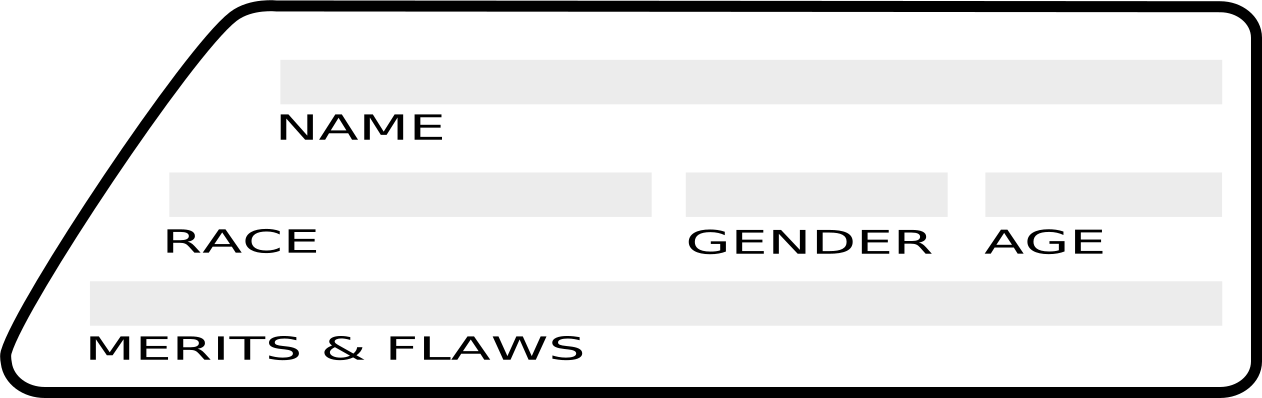
\includegraphics[width=0.95\textwidth]{images/character_base_stats.png}
    \medskip   
\end{column}
\medskip

Name, Geschlecht, Rasse, Alter k"onnen durch den Spieler frei gew"ahlt werden. Die Charaktere werden "ublichereise zwischen 30 und 50 Jahre alt sein. Ein deutlich niedriges oder deutlich h"oheres Alter kann negative Einfl"usse auf k"orperliche Verfassung oder die F"ahigkeiten des Charakters haben. Eine entsprechende Einschr"ankung kann unter MERITS \& FLAWS auf dem Charakter Datenblatt notiert werden. Um die Charaktere dar"uber hinaus lebhafter zu gestalten, kann jeder der Charaktere eine Schw"ache wie Phobie vor gro\3eren Menschenansammlungen, Angst vor engen R"aumen, Sucht nach Aufputschmittel oder Vorurteile gegen Mutanten oder umgekehrt gegen"uber Norms haben.

\newsubsection{Hintergrund}
\begin{column}[l]{0.52}
    Die \cref{sec:character} eingef"uhren Hintergr"unde des Charakters werden im Feld \emph{BACK GROUND} notiert. Die Hintergr"unde beschreiben den individuellen Lebensweg eines Charakters. Hintergr"unde sind jeweils einem der \emph{Attribute} [B]ODY, [E]MPATHY und E[D]UCATION zugeordnet. Die zu einem Attribut zugeordneten speziellen St"arken die sog.~\emph{F"ahigkeiten} beziehen sich immer auf entsprechende Hintergr"unde.
\end{column}
\begin{column}[r]{0.48}
    \centering
    
\includegraphics[width=0.80\textwidth]{images/character_background.png}    
\end{column}

\newsubsection{Attribute und F"ahigkeiten}
Die St"arken eines Charakters werden aufgeteilt nach den Attributen \emph{[B]ODY}, \emph{[E]MPATHY} und \emph{E[D]UCATION} gruppiert. Der Attribute repr"asentieren die Grundf"ahigkeiten des Charakters. Unter den Attributen sind die St"arken des Charakters aufgeteilt in drei \emph{F"ahigkeiten} gelistet. Neben der F"ahigkeiten sind jeweils die Anzahl der W"urfel notiert die f"ur eine Aktionen zur Verf"ugung stehen. Die ausgef"ullte Checkbox neben einem Attribut gibt an, dass f"ur eine Grundf"ahigkeit jeweils ein W"urfel zur Verf"ugung steht. F"ur F"ahigkeiten eines Charakters stehen bis zu drei W"urfel zur Verf"ugung die durch die Checkboxen neben den F"ahigkeiten festgehalten werden. Ein markiertes Dreiecke rechts neben einem Attribut markiert ein Attribut bei dem f"ur F"ahigkeiten bis zu drei W"urfel zur Verf"ugung stehen. Bei Mutanten liegen die F"ahigkeiten f"ur die bis zu drei W"urfel zur Verf"ugung stehen auf dem Attribute BODY. Norms k"onnen frei zwischen EMPATHY und EDUCATION w"ahlen. F"ur F"ahigkeiten k"onnen insgesamt 6 Punkte vergeben werden.
Die F"ahigkeiten eines Charakters beziehen sich immer auf einen entsprechenden Hintergrund. Die Eigenschaft Dexterity eines Piloten erlaubt z.B.~bei der Bedienung eines Raumschiffes oder bei einem Raumspaziergang mehr als einen W"urfel zu werfen w"ahrend ein Schiffstechniker Reparaturen und Modifikationen an einem Schiff kann. In wie weit eine F"ahigkeit auf eine Aktion angewendet werden kann liegt im Ermessen des Spielleiters. Die F"aihigkeiten sind bewusst grob gew"ahlt und "uberschneiden sich in Teilen. Welche F"ahigkeit jeweils angewendet werden kann ergibt sich aus der Aktion die ein Spieler durchf"uhren will.

\begin{column}[l]{0.55}
    F"ur das Attribut BODY, dass k"orperliche Eigenschaften des Charakters darstellt, stehen folgende F"ahigkeiten zur Verf"ugung:

    \begin{description}
        \item[\emph{Fight}] wird im Falle Nah- oder Fernk"ampfen angewendet. Der Hintergrund bestimmt in welcher Kampfart und mit welchen 
            Waffen ein Charakter ausgebildet bzw.~ge"ubt ist.
        \item[\emph{Agility}] umfasst Sportlichkeit und Fingerfertigkeiten und allgemein die eigenschaften der Sinnesorgane dar.
        \item[\emph{Dexterity}] umfasst handwerkliche F"ahigkeiten und die Bedienung von schwerem Ger"at und  die Steuerung von Fahrzeugen 
            und Schiffen. Der Hintergrund bestimmt die Auspr"agung dieses Wertes.
    \end{description}
\end{column}
\begin{column}[r]{0.45}
    \centering
    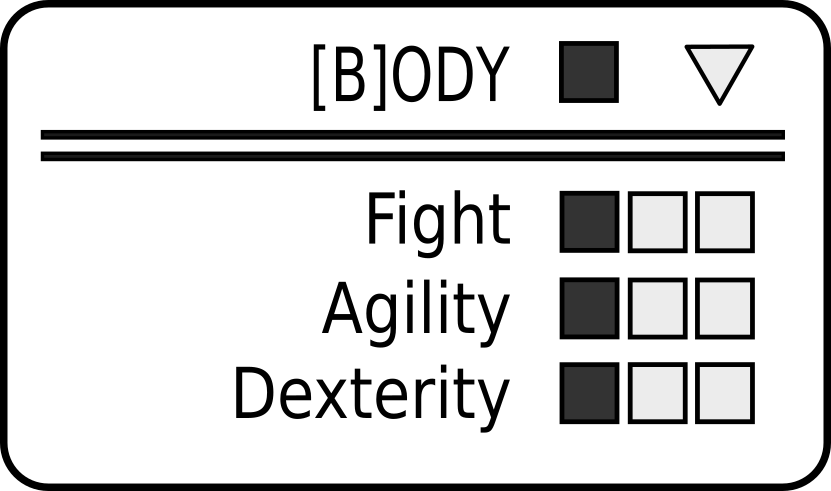
\includegraphics[width=0.80\textwidth]{images/character_body.png}
\end{column}

\begin{column}[l]{0.55}
    F"ur das Attribut EMPATHY, das die Empathy des Charakters darstellt, stehen folgende F"ahigkeiten zur Verf"ugung:

    \begin{description}
        \item[\emph{Knoweledge}] beschreibt das Allgemeinwissen des Charakters dar. Ein Charakter mit ausgepr"agtem Knowelege Wert ist 
            immer bestens informiert.
        \item[\emph{Communication}] beschreibt die Kommunikationsf"ahigkeit des Charakters, d.h.~wie gut er mit anderen Personen umgehen 
            kann.
        \item[\emph{Investigation}] bestimmt wie gut ein Charakter investigative Untersuchungen und Nachforschungen aller Art betreibt.
    \end{description}
\end{column}
\begin{column}[r]{0.45}
    \centering
    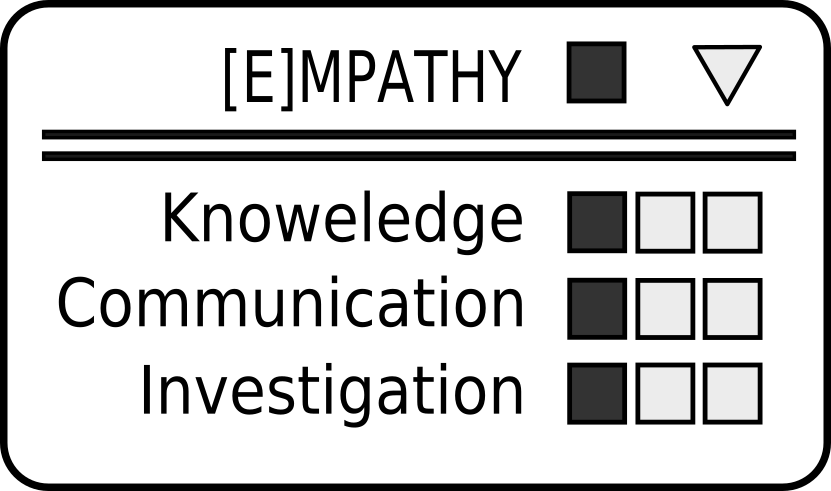
\includegraphics[width=0.80\textwidth]{images/character_empathy.png}
\end{column}

\begin{column}[l]{0.55}
    F"ur das Attribut EDUCATION, das die Bildung des Charakters darstellt, stehen folgende F"ahigkeiten zur Verf"ugung:

    \begin{description}
        \item[\emph{Technics}] beschreibt das Wissen und Verst"andnis f"ur technische Systeme.
        \item[\emph{Medicine}] beinhaltet die F"ahigkeit als Mediziener oder Sanit"ater zu fungieren.
        \item[\emph{Research}] umfasst Forschung auf dem Charakter vertrauten Wissensgebieten.
    \end{description}
\end{column}
\begin{column}[r]{0.45}
    \centering
    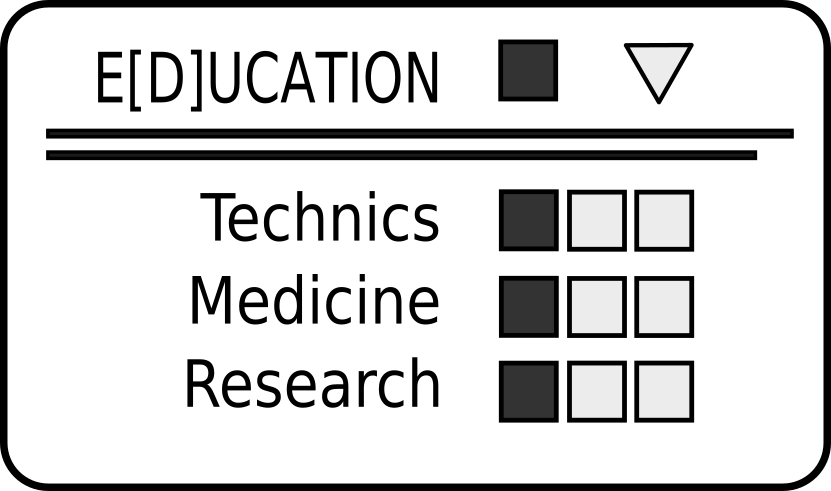
\includegraphics[width=0.80\textwidth]{images/character_education.png}
\end{column}

\medskip
\begin{ruleexample}
    Die Gruppe fl"uchtet von einer Orbitalstation in ein angedocktes Wartungsshuttle um mit diesem auf einem Mond im Umfeld des Planeten zu landen. Das Shuttle kann nicht aus eigener Kraft zum Mond "uberwechseln. Ein Parabelflug mit verscheidenen Meteoren in der Umgebung soll genutzt werden das Shuttle zu beschleunigen und auf eine passende Flugbahn zu bringen. Hier m"ussen alle Charaktere zusammen arbeiten:

\begin{description}
        \item[Celine ({Hintergrund Mathematikerin [D]})] berechnet "uber ihrer mit drei W"urfeln ausgepr"agten F"ahigkeit Research eine 
            m"ogliche Flugbahn.
        \item[Henk ({Hintergrund Navigator [E)})] nutzt die durch Celine berechnete Flugstrecke um mit Knoweledge die Flugparameter zu 
            bestimmen.
        \item[Tom ({Hintergrund Shuttlepilot [B]})] bewegt das Shuttle aus dem Landungsdock und in die inital berechnete Flugbahn.
    \end{description}
\end{ruleexample}

\newsubsection{Waffen}
\begin{column}[l]{0.55}
    Im Bereich \emph{WEAPONS} k"onnen die Waffen die dem Charakter zur Verf"ugung stehen eingetragen werden. Spielercharaktere besitzen in den meisten F"allen eine halbautomatische Handfeuerwaffe. Je nach Profession stehen mehr Waffen zur Verf"ugung. Die Waffen sind mit dem Spielleiter abzusprechen. 
\end{column}
\begin{column}[r]{0.45}
    \centering
    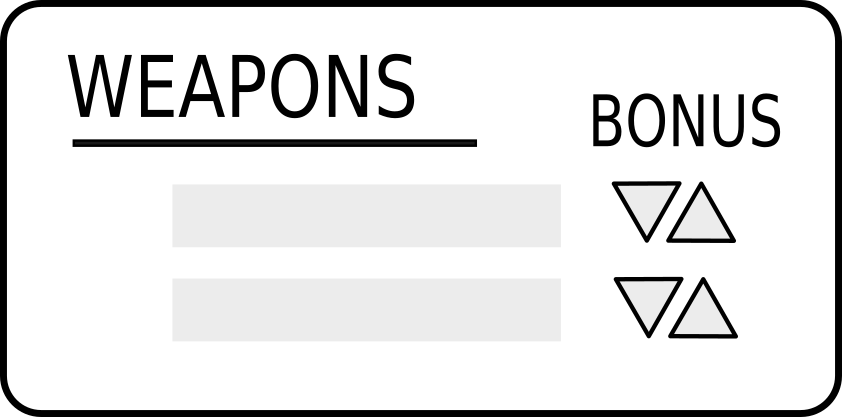
\includegraphics[width=0.80\textwidth]{images/character_weapons.png}
\end{column}
\medskip

Eine Auswahl an Waffen steht unter dem Kapitel "`Waffen"' zur Verf"ugung. Dort sind auch spezielle Eigenschaften der Waffen notiert. Neben der Waffe sind auf dem Charakterblatt zwei Dreiecke angegeben. Bei Waffen die schwer zu bedienen sind wird das nach unten zeigende Dreieck ausgef"ullt. Bei einer schwer zu bedienenden Waffe werden Angriffe mit einem W"urfel weniger (\emph{Malus}) minimal aber mit einem W"urfel gew"urfelt. Bei Waffen die eine erh"ohte Trefferchange aufweisen wird das nach oben zeigende Dreieck ausgef"ullt (\emph{Bonus}). Bei Waffen mit einer erh"ohten Trefferchange wird mit einem W"urfel mehr gew"urfelt.

\newsubsection{K"orperpanzerung}
\begin{column}[l]{0.55}
    Im Bereich \emph{ARMOR} werden die dem Charakter zur Verf"ugung stehenden K"orperpanzerungen und spezielle Kleidung wie ein Raumanzug eingetragen. Panzerung wie eine schusssichere Weste ist kein allt"agliches Kleidungsst"uck und wird dadurch normalerweise nicht getragen. 
\end{column}
\begin{column}[r]{0.45}
    \centering
    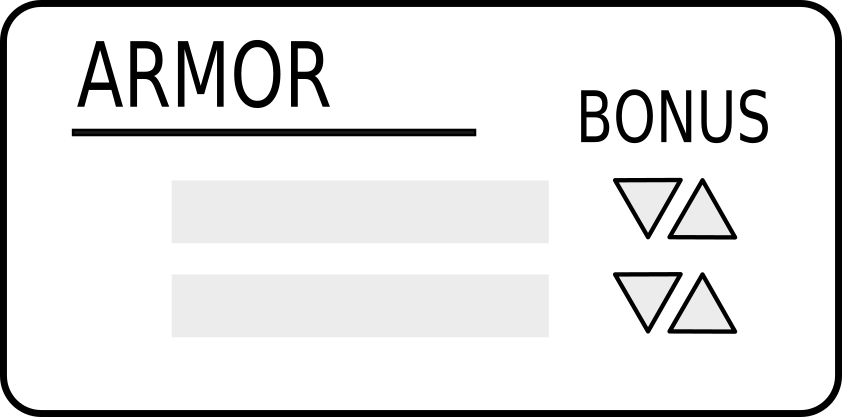
\includegraphics[width=0.80\textwidth]{images/character_armor.png}
\end{column}
\medskip

Eine Auswahl an K"orperpanzerungen sind im Kapitel "`Technologie"' angegeben. Dort sind auch spezielle Eigenschaften von Panzerungen angegeben.  Neben der Kleidung sind auf dem Charakterblatt zwei Dreiecke angegeben. Bei Kleidung die den Charakter stark behindern und gleichzeitig nicht ausreichend sch"utzt wird das nach unten zeigende Dreieck ausgef"ullt. Bei einer behindernden Kleidung wird die Verteidigung mit einem W"urfel weniger gew"urfelt (\emph{Malus}). Bei Panzerung die den Charakter an wichtigen K"orperteilen gut sch"utzt wie eine Schusssichere Weste oder ein Gefechtspanzer wird das nach oben zeigende Dreieck ausgef"ullt. Bei solchen K"orperpanzern wird die Verteidigung mit einem W"urfel mehr gew"urfelt (\emph{Bonus}).

\newsubsection{Inventar}
\begin{column}[l]{0.55}
    Im Bereich \emph{INVENTORY} sind die pers"onlichen Habseligkeiten des Charakters notiert. Das Inventar umfassen auch K"orpermodifikationen wie Headware und modifizierte Gliedma\3en. Charkater sind "ublicherweise st"andig unterwegs. Die Gegenst"ande unter INVENTORY sind die Gegenst"ande die der Charakter "ublichweise bei sich tr"agt. Die Gegenst"ande werden zusammen mit dem Spielleiter unter Ber"ucksichtigung des Werdegangs festgelegt.
\end{column}
\begin{column}[r]{0.45}
    \centering
    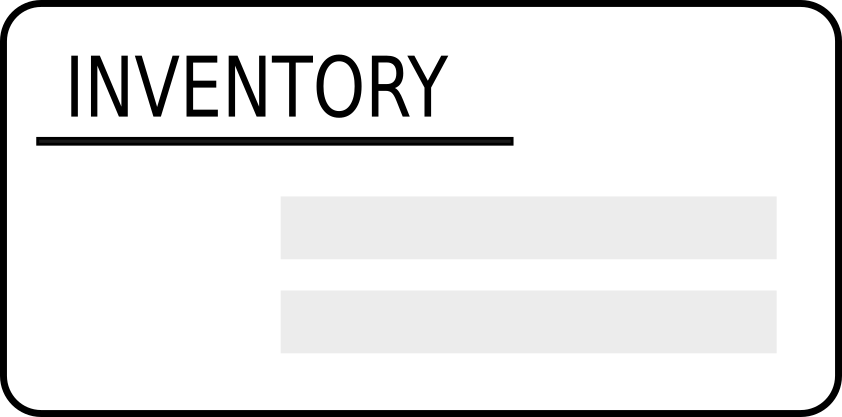
\includegraphics[width=0.80\textwidth]{images/character_inventory.png}
\end{column}
  
\newsection{Rassenbesonderheiten}

Den Spieler stehen Norms, Alpha-Mutanten und Omega-Soldaten zu Auswahl. Bez"uglich dem Regelwerte gelten folgende Besonderheiten.

\begin{description}
    \item[Norms] Norms sind normale Menschen, im Falle der Charaktere gebildete Menschen mit einer Hochschulbidung im Zivilen oder 
        milit"arischen Sektor. Ihr St"arke liegt dadurch beim Attribut \textbf{EDUCATION}. In diesem Bereich k"onnen bis zu zwei Punkte bei den F"ahigkeiten vergeben werden. Die Charaktere k"onnen in ihrer Laufbahn eine leitende Stelle eingenommen haben und werden von Konzernmitarbeitern als Ansprechpartner wahrgenommen. Die Charaktere h"atten die M"oglichkeit hochwertige K"orpermodifikationen durchf"uhren zu lassen. Norms besitzen einen familier"aren Hintergrund auch wenn der Kontakt abgebochen ist bestehen wenn n"otig Kontakte aus Schulzeit und Hochschulzeiten.
    \item[Alpha-Mutanten] Alpha-Mutanten sind in einer Zuchtfarm auf dem Mars als Arbeiter ausgebildet worden. Die geh"oren der
        Arbeiterklasse an. Sie sind handwerklich gut ausgebildet. Aufgrund ihres genetischen Zuchtmaterials sind sie gr"o\3er, st"arker und widerstandsf"ahiger als Norms. Bei k"orperlichen T"atigkeiten wie auch bei K"orperbelastungen sollten diese k"orperlichen Besonderheiten bei den Auswirkungen von Aktionen ber"ucksichtigt werden. Die m"ogliche St"arke der Alpha-Mutanten liegt damit auf dem Attribut \textbf{BODY}. Bei den entsprechenden F"ahigkeiten k"onnen dadurch jeweils bis zu zwei Punkte ausgegeben werden. Alpha-Mutanten werden als Teil der Zivilgesellschaft wahrgenommen und werden aufgrund ihrer meist umg"anglichen Art im extraterrestrischen Umfeld freundschaftlich behandelt und als Zuverl"assig gesch"atzt. Alpha-Mutanten sind im Normalfall mit dem Leben in Schwerelosigkeit vertraut. Alpha-Mutanten haben eine handwerkliche und meist eine logistische Ausbildung erhalten. Alpha-Mutanten haben innerhalb ihrer Zuchtreihe jeweils eine eigene Sprache erlernt und k"onnen sich damit mit ihren "`Artgenossen"' aber auch anderen Alpha-Mutanten unverst"andlich f"ur Norms und Omega Mutanten unterhalten. 
    \item[Omega Mutanten] Omega Mutanten sind entweder auf dem Mars oder in Zuchtfarmen im erdnahen Orbit aufgewachsen. Sie sind deutlich   
        gr"o\3er, st"arker und widerstandsf"ahiger wie Alpha-Mutanten und Norms. Bei allen k"orperlichen Aktionen und Folgen von Verletzungen m"ussen diese "uberlegenen Eigenschaften ber"ucksichtigt werden. Ihre St"arke im W"urfelsystem liegt wie bei Alpha-Mutanten im Sttribut \textbf{BODY}. Hier k"onnen auf alle F"ahigkeiten bis zu zwei Punkte vergeben werden. Omega-Soldaten werden von klein auf auf den Krieg vorbereitet und ausgebildet. Nah- und Fernkampff"ahigkeiten sind vorauszusetzen. Omega Mutanten sind mit milit"richen K"orpermodifikationen ausgestattet. Omega Mutanten haben eine strategische und logistische Ausbildung f"ur Krisensituationen erhalten. Sie sind f"ur die m"uhelose Bewegung in Schwerelosigkeit vorbereitet. Sie haben auch eine medizinische Ausbildung als Sanit"ater erhalten. Viele Omega Mutanten sind ausgebildete Piloten oder haben eine Ausbildung als Schiffskommandant absolviert. Aufgrund ihrer genetischen Programmierung sind Omega Mutanten leicht reizbar und gehen schnell offensiv mit einer Provokation oder einer Bedrohung um. Sie unterliegen deshalb dem \textbf{FLAW} "`reizbar"'. Von nicht Omega Mutanten werden sie oft als militanten Bedrohung wahrgenommen.
\end{description}

\newsection{Kampf und Verletzungen}
Im Alltag eines Helden l"asst sich eine Auseinandersetzung nicht immer friedlich l"osen. Es kommt zum Kampf. In diesem Kapitel werden K"ampfe zwischen Personen und die Auswirkung von Verletzungen beschrieben.

Eine Aktion in einem Kampf umfasst eine \emph{Kampfszenen}. Eine solche Kampfszene kann eine oder mehrere Schlagabtausche, Schusswechsel und Ausweichman"over enthalten. Der Spieler beschreibt was sein anvisiertes Ziel in der Kampfszene ist. Will er einen oder mehrere Gegner zu Fall bringen, will er in eine Deckung fl"uchten oder einen fl"uchtenden Gegner niederschie\3en. 

Darauf hin wird gew"urfelt. K"ampfe sind im Normalfall vergleichende W"urfe. Entschlie\3t sich ein Charakter seinen Gegner \textbf{anzugreifen} w"urfelt er mit seiner F"ahigkeit \textbf{Fight}. Beschr"ankt sich der Charakter auf \textbf{Verteidigung} wird mit der F"ahigkeit \textbf{Agility} gew"urfelt. Der Erfolg einer Aktion wird jeweils durch den W"urferfolg des Gegners reduziert unabh"angig davon ob der Gegner selbst angreift.

\begin{ruleexample}
    Hektor und der Minenarbeiter Fury ein kr"aftiger Alpha-Mutant sind sich ins Gehege gekommen. Fury schl"agt zu. Hektor sieht sich unterlegen und versucht zu fliehen. Fury w"urfelt mit Fight eine \ssdice{6}, voller Erfolg. Hektor w"urfelt mit Agility ebenfalls ein \ssdice{6}, voller Erfolg. D.h. Furys Angriff sind ein Teilerfolgt. Furys schl"age sind kr"aftig und gut gezieht aber Hektor schafft es immer wieder gekonnt abzutauchen und steckt nur leichte treffer ein. Hektor auf der anderen Seite schafft es mit einem Teilerfolg ebenfalls nicht zu fliehen kann aber am Ende zumindest Abstand zwischen sich und den Gegner zu bringen und kann nun versuchen Fury zu beruhigen.
\end{ruleexample}

\newsubsection{Kampf mit mehreren Personen}
Oft sind an einem Kampf mehrere Personen beteiligt. Wie bei anderen Aktionen k"onnen Angreifer oder Verteidiger ihren Angriff b"undeln um ihre Erfolgschancen zu erh"ohen. Sie k"onnen dabei ihren Angriff oder ihre Verteidigung zusammen auf einen Gegner richten. Die W"urfel aller an einer Aktion beteiligten werden dann als ein W"urfelpool zusammen gew"urfelt. F"ur den W"urfelwurf des Gegners "andert sich nichts. Richtet ein Angreifer auf der anderen Seite seinen Angriff auf mehrere Personen b"undeln damit die Gegner im Gegenzug dazu ihren Angriff oder ihre Verteidigung.

\newsubsection{Nahkampf}
Im Nahkampf treten sich Personen waffenlos oder mit Hieb oder Stichwaffen entgegen. Ein Kampf wird rundenweise als vergleichender W"arfelwurf ausgefochten.

Exemplarisch verschiedene Nahkampfsituationen:

\begin{description}
    \item[Fixieren] Ein Angriff um einen Gegner festzuhalten und Bewegungsunf"ahig zumachen. Um einen Gegner festzuhalten um ihn    
        kampfunf"ahig zu mache wird ein \textbf{voller Erfolg} ben"otigt. Ein Teilerfolg k"onnte bedeuten, dass der Gegner zwar nicht fl"uchten kann aber noch lange nicht kampfunf"ahig ist.
    \item[Entwaffnen] Dem Gegner eine Waffe zu entrei\3en oder sie davon zu schlagen erfordert einen \textbf{vollen Erfolg}. Ein Teilerfolg 
        sollte zumindest sich aus der Schusslinie der Waffe zu bringen.
    \item[Schl"agerei] Ein Nahkampf zwischen mehreren Personen sollte sich aufgrund der Enge auf vier Personen beschr"anken die in direktem 
        Kontakt zu einander stehen.
\end{description}


\newsubsection{Fernkampf}
Fernkampf bezieht sich auf Angriffe mit Schusswaffen, Granaten und Plasmaschleudern. Der Angreifer w"urfelt auf \textbf{Fight} um anzugreifen.

Folgende Besonderheiten m"ussen ber"ucksichtig werden:

\begin{description}
    \item[Gegenangriff] Ein Angreifer der einen Gegner im Fernkampf bek"ampft also z.B.~selbst eine Schusswaffe abfeuert kann im Normalfall 
        nicht ausweichen. Im besten Fall kann er einen Risikowurf versuchen um beim Ausweichen noch gezieht schie\3en zu k"onnen.
    \item[Ausweichen] Um einem Fernkampfangriff auszuweichen mu\3 der Verteidiger bereits in Bewegung sein, Haken schlagen, in Dekung 
        hechten. Einem Fernkampfangriff wird mit \textbf{Agility} ausgewichen. 
    \item[Point-Blank] Ein Angreifer der einen Gegner auf eine Distanz von wenigen Metern bedroht hat leichtes 
        Spiel. Er w"urfelt seinen Angriff mit einem \textbf{Alltagswurf}. Der Angegriffene kann einen Nahkampf Gegenangriff versuchen oder sich mit einer schnellen Bewegung aus der Schusslinie zu bringen. Er w"urfelt einen \textbf{Einfachen Wurf} als Verteidigung.
    \item[Deckung] Ein Verteidiger der in teilweiser Deckung steht is schwerer zu treffen. Er w"urfelt einen \textbf{Alltagswurf} als 
        Verteidigung.
\end{description}

\newsubsection{Schaden}
Bei K"ampfen oder auch anderweitig kann ein Charakter verletzt werden. Verletzungen werden nicht wie in anderen Rollespielen mittels Lebenspunkten festgehalten. Statdessen bestimmt der Spielleiter Aufgrund des Angriff, der Verteidigung und der Panzerung des angegriffenen die aufgetretene Verletzung. 

\begin{column}[l]{0.58}
    Wird der Charakter im Kampf oder bei einer sonstigen T"atigkeit verletzt wird unter \emph{DAMAGE} die zugezogenen Verletzungen notiert. 
    Es wird zwischen \textbf{leichtem und schwerem Schaden} unterschieden. Bei schweren Verletzungen ist ein Konstitutionswurf notwendig damit der Charakter weiter Handlungsf"ahig bleibt. Werden schwere Sch"aden nicht behandelt oder setzt sich der Charakter weiter k"orperlicher Belastung aus kann er in der Folge ebenfalls Handlungsunf"ahig werden. In disesem Fall k"onnen weitere Konstitutionsw"urfe eingefordert werden. Ein Konstituionswurf ist in der Regel ein \textbf{einfacher Wurf} auf \emph{CONST}.
\end{column}
\begin{column}[r]{0.42}
    \centering
    
\includegraphics[width=0.80\textwidth]{images/character_damage.png}

    
\includegraphics[width=0.80\textwidth]{images/character_const.png}
\end{column}
\smallskip

Schwere Verletzungen in Verbindung mit einem nicht erfolgreichen Konstitutionswurf k"onnen zum Tod f"uhren. Die Verletzung mu\3 sofort behandelt werden. Ein sterbender Charakter kann wieder belebt werden. Die Medizin ist im 23ten Jahrhundert ist wie im Kapitel "`Helden"' beschrieben weit fortgeschritten. K"orpermodifikation k"onnen dabei helfen den Charakter am leben zu halten. Ein erste Hilfe Kit enth"alt Ausr"ustung zur Wiederbelebung und Stabilisierung.


\newsubsection{Panzerung}
Um sich gegen Angriffe durch Schusswaffen oder bei einem Nahkampf zu sch"utzen kommen Panzerungen ins Spiel. Um bei einer Panzerung gr"o\3eren Schaden anzurichten m"ussen schlechter gesch"utzte K"orperteile getroffen werden. F"ur einen gezielten Treffer ist ein \textbf{voller Erfolg} notwendig.

Folgende Panzerungen kommen im C23 Universum zum Einsatz:

\begin{description}
    \item[Schusssichere Weste und Helm] Einen effektiven Schutz gegen Feuerwaffen bieten bereits eine schusssichere Weste und ein Helm. Sie 
        sch"utzen den Torso und Teile des Kopfes effektiv vor Stichwaffen und Projektilen und bieten besseren Schutz vor stumpfen Waffen. Ein Treffer auf Weste und Helm hinterl"asst Prellungen und kann die Zielperson zum Straucheln und nach Luft schnappen bringen hat aber sonst keine Wirkung.
    \item[Kampfanzug] Noch besseren Schutz bietet eine Kampfanzug der auch den Rest des K"orpers inklusive Kopf sch"utzt. Ein Kampfanzug 
        bietet an allem K"orperteilen besseren Schutz aber er sch"utzt nicht vollst"andig vor Schusswaffen oder Schl"agen. Bewegliche Teile wie Gliedma\3en sind schlechter gesch"utzt. Bei einem Treffer mu\3 der Schutz an allen K"orperbereichen mit ber"ucksichtigen.
    \item[Servopanzer] Ein Servopanzer ist ein hydraulisch unterst"utztes ganzk"orper Exoskelett mit eingebautem Raumanzug und 
        Waffensystem. Treffer einer Nahkampfwaffe wie auch durch ein Bolzenpistole sind an den gut gesch"utzten K"orperbereichen wirkungslos. Auch weniger gesch"utzte Teile sind deutlich besser gesch"utzt wie bei einem Kampfanzug. Ein K"ampfer in einem Servopanzer kann auch kaum zu Fall gebracht werden.
\end{description}

Schwerere Waffen:

\begin{description}
    \item[Railguns] Railguns verschie\3en in der Regel gr"o\3ere Projektile in einem Feuersto\3. Ein ungesch"utztes K"orperteil zu treffen 
        oder eine R"ustung zu durchschlagen ist damit leicher wie mit einem Bolzenpistole.
    \item[Granaten] Geworfene Granaten und Granatwerfer treffen ihren Gegner mit Splittern und einer Explosion.
    \item[Plasmaschleuder] Eine Plasmaschleuder ist eine Waffe mit R"uckentank die einen hochenergetischen Feuerball abfeuert der sich auch 
        durch ma\3iven Stahl hindurch bennen kann. Nach abschie\3en von Plasmapartikeln ben"otigt die Waffe in etwa eine Minute um wieder einsatzbereit zu sein. Eine Plasmaschleuder hat je nach Abstand einen Trefferwinkel von 1.5 bis zu 2 Metern.
\end{description}

\newsection{Cyberkampf}\anchor{sec:cyberkampf}
Cyberkampf ist Kampf im ComNetz. In das ComNetz kann sich ein Charakter mittels eines station"aren Terminals, einem Comnputer oder seinem ComLink einloggen. Weitaus effektiver ist jedoch das vollsensorische Eintauchen mittels Kontrollmodul. Der Charakter taucht dann mit all seinen Sinnen in die virtuelle Realit"at des Datennetztes. Mittels Gedankenkontrolle lassen sich dann Befehle absetzen. Informationen k"onnen durch alle Sinnesorgane aufgenommen. F"ur diese Art des Einstiegs ins Netz ist eine breitbandige Verbindung notwendig. 

F"ur die Informationsbeschaffung oder "uberwachung im Netz k"onnen Agentensysteme mit Auftr"agen losgeschickt werden. 

Andere Systeme im Netz k"onnen "uber eine Cyberattacke auch unterst"utzt durch Agentensysteme und Viren angegriffen werden. Auch der ComLink zusammen mit dem Personal Area Network (PAN) eines Netzteilnehmers oder auch das Kontrollmodul sind Systeme im Netz die angegriffen werden k"onnen. Eingespeiste Viren k"onnen die Headware des Teilnehmers beeintr"achtigen und dadurch Sinneswahrnehmungen beeinflussen, Hormoneinspei\3ungen einleiten oder k"unstliche K"orperfunktionen beeinflussen. Firewallsoftware sch"utzt alle Formen von Systemen im Netz vor Cyberattacken.

Eine Cyberattacke wird wie eine physikalische Attacke durch vergleichende W"urfelw"urfe durchgef"uhrt. Cyberangriffe und das Programmieren von Viren und Agentensystemen wird mit der F"ahigkeit \textbf{Technics} gew"urfelt.

\newsection{Psychonauten}
Psychonauten wie im Kapitel "`Technologie"' beschrieben k"onnen in das Gehirn einer anderen Person "uber ein entsprechendes Equipment eindringen. "Ahnlich wie beim Eintauchen in das ComNetz besteht kann eine vollsensorische Verbindung zwischen beiden Personen. Der Psychonaut denkt quasi im Gehirn des anderen mit. Der Psychonaut dringt zun"achst in die oberfl"achliche Gedanken des Hier und Jetzt ein kann aber danach tiefer in das Unterbewusstsein eintauchen und Wissen und Gef"uhle erkunden. Der Psychonaut kann dabei spezifische Informationen anfragen und nimmt dann "ahnlich wie in einem Traum Bilder und Sinneseindr"ucke wahr. Ein Gehirnscan wird mit der F"ahigkeit \textbf{Research} ge"urfelt. Das Opfer des Gehirnscans kann sich mit einem Wurf auf \textbf{Empathy} verteidigen, im Falle eines Psychonauten ebenfalls mit \textbf{Research}. Ein Gehirnscan ist gef"ahrlich f"ur den gescanten wie auch f"ur den Psychonauten. Wehrt sich der gescante bei einem Tiefenscan und w"urfelt einen Mi\3erfolg kann sein Gehirn psychischen Schaden nehmen. Auf der anderen Seite ist die Gehirnverbindung bidirektional. Ein Mi\3erfolg bei einem Scan kann dazu f"uhren, da\3 der gescante selbst Informationen aus dem Gehirn des Psychonauten erf"ahrt oder der Psychonaut psychischen Schaden nimmt.

\newsection{Raumkampf}
Bei einer Auseinandersetzung im Weltall k"onnen Auseinandersetzungen mit den im Kapitel "`Raumschiffe"' beschriebenen Schiffsklasssen ausgefochten werden. Den Charakteren werden "ublicher F"ahren oder Frachter eventuell auch eine Korvette zur Verf"ugung stehen. Korvetten, J"ager sind mit Railguns oder Gau\3kanonen ausgestatttet. gelegentlich auch mit Raketen oder Torpodos. Mehrere 100m gro\3e Gro\3kampfschiffe wie Fregatten, Schlachkreuzter und Flottentr"ager sind in jedem Fall mit Railguns oder Gau\3kanonen, Raketen und Torpedos ausgestattet. Railguns auf Grund ihrer hohen Feuerfrequenz werden bei Schiffen gr"o\3er als ein Korvette prim"ar als Verteidigungswaffen genutzt. Sonden k"onnen als Aufkl"arungsger"ate zur visuellen Analyse "uber gro\3e Entfernunungen genutzt werden.

Ein Schiff besteht dominierend aus einem Fusionstriebwerk als Hauptantrieb einer Reihe von Steuerungstriebwerken, einem Lebenserhaltungssystem und einer gro\3en Menge von Sensoren. Alle Systeme bis auf den Antrieb sind mit Redundanzsystemen ausgestattet. Da die Mannschaft im freien Raum komplett auf sich selbst gestellt ist k"onnen ein Gro\3teil der Technik eines Schiffs autonom repariert und ausgetauscht werden. Ein Weltraumspaziergang ist f"ur die Crew eines Schiffes kein au\3ergew"ohnlicher Vorfall und kann auch bei hoher Fluggeschwindigkeit durchgef"uhrt werden. Einen gro\3en Teil der Zeit befindet sich ein Schiff im Driftflug, d.h. mit ausgeschalteten Triebwerken. Es herrscht Schwerelosigkeit an Bord. Nur unbedingt notwendige Systeme sind aktiv. Der Raktor des Haupttriebwerks kann innerhalb weniger Minuten hochgefahren werden und bietet dann ein vielfaches an Energie gegen"uber einem klassischen Raketenantrieb. Ein Fusionstriebwerk wie auch die Steuerd"usen ben"otigen Treibmasse allerdings in deutlich wenigerem Umfang wie bei heutigen Raketen.

Im freien Raum sind die Gegebenheiten viele Stunden vor dem Zusammentreffen einsehbar. Der taktische Computer des Schiffes zeigt alle "uber die Sensorik erfassbaren Daten in 3D Ansicht an. Auf dem Display sind die derzeitigen und prognostizierbaren Flugbahnen von Schiffen, Planenten, Monden und anderen Himmelsk"orpern einsehbar sofern sie erfasst werden k"onnen.

Ein strategisches Planen von Raumk"ampfen auf einem Schlachtplan w"are m"oglich. Ist der Kampf aber nicht der Fokus der Geschichte sollten nur einige kurze Kampfszenen ausgespielt werden. Die Schiffskontrolle und die Kontrolle der Waffensysteme wird dabei durch die F"ahigkeit \textbf{Dexterity} gew"urfelt. Ein f"ur eine Reparatur notwendiges Fachwissen wird durch die F"ahigkeit \textbf{Technics} abgebildet. F"ur Flugplanung und Raumkathographie wird die F"ahigkeit \textbf{Knoweledge} ben"otigt. F"ur einen Au\3enspaziergang w"urfelt man auf \textbf{Dexterity}.
